%%%%%%%%%%%%%%%%%%%%%%%%%%%%%%%%%%%%%%%%%%%%%%%%%%%%%%%%%%%%%%%%%%%%%%%%%%%%%%%%%%%%%%%
%%%%%%%%%%%%%%%%%%%%%%%%%%%%%%%%%%%%%%%%%%%%%%%%%%%%%%%%%%%%%%%%%%%%%%%%%%%%%%%%%%%%%%%
% 
% This top part of the document is called the 'preamble'.  Modify it with caution!
%
% The real document starts below where it says 'The main document starts here'.

\documentclass[12pt]{article}

\usepackage{amssymb,amsmath,amsthm}
\usepackage[top=1in, bottom=1in, left=1.25in, right=1.25in]{geometry}
\usepackage{fancyhdr}
\usepackage{enumerate}
\usepackage{listings}
\usepackage{graphicx}
% Comment the following line to use TeX's default font of Computer Modern.
\usepackage{times,txfonts}

\newtheoremstyle{homework}% name of the style to be used
  {18pt}% measure of space to leave above the theorem. E.g.: 3pt
  {12pt}% measure of space to leave below the theorem. E.g.: 3pt
  {}% name of font to use in the body of the theorem
  {}% measure of space to indent
  {\bfseries}% name of head font
  {:}% punctuation between head and body
  {2ex}% space after theorem head; " " = normal interword space
  {}% Manually specify head
\theoremstyle{homework} 

% Set up an Exercise environment and a Solution label.
\newtheorem*{exercisecore}{Exercise \@currentlabel}
\newenvironment{exercise}[1]
{\def\@currentlabel{#1}\exercisecore}
{\endexercisecore}

\newcommand{\localhead}[1]{\par\smallskip\noindent\textbf{#1}\nobreak\\}%
\newcommand\solution{\localhead{Solution:}}

%%%%%%%%%%%%%%%%%%%%%%%%%%%%%%%%%%%%%%%%%%%%%%%%%%%%%%%%%%%%%%%%%%%%%%%%
%
% Stuff for getting the name/document date/title across the header
\makeatletter
\RequirePackage{fancyhdr}
\pagestyle{fancy}
\fancyfoot[C]{\ifnum \value{page} > 1\relax\thepage\fi}
\fancyhead[L]{\ifx\@doclabel\@empty\else\@doclabel\fi}
\fancyhead[C]{\ifx\@docdate\@empty\else\@docdate\fi}
\fancyhead[R]{\ifx\@docauthor\@empty\else\@docauthor\fi}
\headheight 15pt

\def\doclabel#1{\gdef\@doclabel{#1}}
\doclabel{Use {\tt\textbackslash doclabel\{MY LABEL\}}.}
\def\docdate#1{\gdef\@docdate{#1}}
\docdate{Use {\tt\textbackslash docdate\{MY DATE\}}.}
\def\docauthor#1{\gdef\@docauthor{#1}}
\docauthor{Use {\tt\textbackslash docauthor\{MY NAME\}}.}
\makeatother

% Shortcuts for blackboard bold number sets (reals, integers, etc.)
\newcommand{\Reals}{\ensuremath{\mathbb R}}
\newcommand{\Nats}{\ensuremath{\mathbb N}}
\newcommand{\Ints}{\ensuremath{\mathbb Z}}
\newcommand{\Rats}{\ensuremath{\mathbb Q}}
\newcommand{\Cplx}{\ensuremath{\mathbb C}}
%% Some equivalents that some people may prefer.
\let\RR\Reals
\let\NN\Nats
\let\II\Ints
\let\CC\Cplx

%%%%%%%%%%%%%%%%%%%%%%%%%%%%%%%%%%%%%%%%%%%%%%%%%%%%%%%%%%%%%%%%%%%%%%%%%%%%%%%%%%%%%%%
%%%%%%%%%%%%%%%%%%%%%%%%%%%%%%%%%%%%%%%%%%%%%%%%%%%%%%%%%%%%%%%%%%%%%%%%%%%%%%%%%%%%%%%
% comment 
% The main document start here.

% The following commands set up the material that appears in the header.
\doclabel{Math 426: Homework 1 (Part A)}
\docauthor{Stefano Fochesatto}
\docdate{\today}

\begin{document}
\textbf{Part A (Matlab Tutorial)}
\begin{exercise}{5}
let $p(t) = -1+3t-2t^3$ -that is, $p$ is a polynomial. Use Matlab to compute the value of $p$
at each of the entries of $x$. The first entry of this matrix should be $p(7)$ since the first entry of $x$ is 7. 
The last entry of this matrix should be $p(2)$ since 2 is the last entry of $x$ \\

\textbf{Solution:}
\lstinputlisting{myDiaryFile}
Using the $polyval$ function:
\lstinputlisting{myDiaryFile1}
\end{exercise}

\vspace{1in}



\begin{exercise}{7} Plot the curves $y = Ce^x$ for $C = 1$,$C = 1/2$, $C = 0$, $C = -1/2$ and $C = -1$ 
  the range $-1 \leq x \leq 1$ all in the same figure. Add a helpful legend in your plot.\\

  \textbf{Solution:}
  \lstinputlisting{myDiaryFile2}
  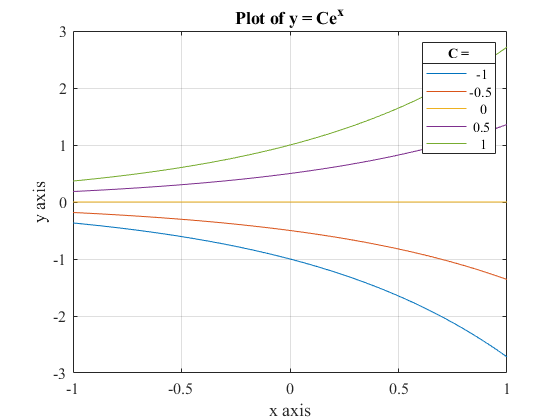
\includegraphics[width=\textwidth]{ex7.png}

  
\end{exercise}

\vspace{1in}


\begin{exercise}{9} Let,
  \begin{equation*}
    logistic(x) = \frac{1}{1+e^{-x}}.
  \end{equation*}

  \begin{enumerate}
    \item Following the example from section use matlab to define a function $logistic$ for this function.\\\\
    \textbf{Answer:}
    \lstinputlisting{myDiaryFile3}

    
    \item Verify that your function works correctly b computing $logistic(0), logistic(1)$ and $logistic([0,1])$. Do you obtain the right answers? (Hint: if you have a error when you test with vector input think about dot operators)\\\\
    \textbf{Answer:}
    \lstinputlisting{myDiaryFile4}
    Note the .\string^(-1) notation. When applied to a vector .\string^(-1) inverts each entry individually, achieving the desired result. Also note that the notation $1./$ would achieve the same result.

    \item Plot the logistic function over the range $-2 \leq x \leq 2$. Add a red square or diamond that marks the point $(1, logistic(1))$ \\\\
    \textbf{Answer:}
    \lstinputlisting{myDiaryFile6}
    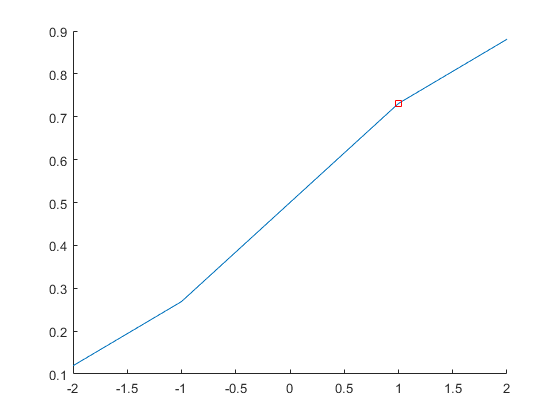
\includegraphics[width=\textwidth]{ex9.png}
  \end{enumerate}
  



\end{exercise}
\end{document}